
\documentclass[11pt]{article}


\usepackage[utf8x]{inputenc}
\usepackage{hyperref}
\usepackage{amsmath}
\usepackage{amssymb} 
\usepackage{textcomp}
\usepackage[frenchb]{babel}
\usepackage{natbib} 
\usepackage{hyperref} 


\usepackage{graphicx}
\graphicspath{{./}{./1_semester}{./analyse}{./methodology}}

\usepackage[top=3.5cm, textheight=21.5cm, textwidth=17cm, footskip=1cm, headsep=1cm]{geometry}

\usepackage{fancyhdr}
\pagestyle{fancy}
\fancyhf{}
\lhead{\fontsize{10pt}{12pt}\selectfont Le secret bancaire suisse au XXe siècle dans le
\textit{Journal de Genève} et la \textit{Gazette de Lausanne}}
\rhead{}
\rfoot{\fontsize{10pt}{12pt}\selectfont \thepage}
\lfoot{\textit{\fontsize{10pt}{12pt}\selectfont Yann Bolliger, Pietro Carta et Romain Mendez}}


\title{
   Le secret bancaire suisse au XXe siècle dans le
  \textit{Journal de Genève} et la \textit{Gazette de Lausanne}
}
\author{Yann Bolliger, Pietro Carta et Romain Mendez}

\begin{document}
  
\pagestyle{empty}

\begin{figure}
\centering

\includegraphics[width=0.25\textwidth]{logo.png}
\vspace{-1cm}
\end{figure}

\maketitle

\newpage

\pagestyle{fancy}
\section{Contexte historique}

La place financière suisse a vu une énorme croissance presque non perturbée tout
au long du XXème siècle. Cela a été possible grâce à la neutralité et la
stabilité de la Suisse notamment en période de guerre mais surtout aussi grâce
au  ``secret bancaire'' \citep[p. 512]{Mazbouri12}. 
Le terme secret bancaire apparaît dans la presse romande dans les années 20,
ce que l'on peut observer dans les archives du \textit{Journal de Genève (JDG)} et 
de la \textit{Gazette de Lausanne (GDL)}.

Ce dernier est déjà une
pratique des banques suisses au XIXème siècle quand les grandes
banques\footnote{Union de Banques Suisses, Schweizerische Kreditanstalt (Crédit
Suisse), Schweizerische Volksbank, Banque Leu, Eidgenössische Bank, Société de
Banque Suisse, Banque Commerciale de Bâle et le Comptoir d’Escompte} commencent
à dominer la place financière suisse. Ces banques-là profitent considérablement
des afflux de capitaux étrangers. Pendant la Grande Guerre les banques utilisent
le secret bancaire pour attirer les capitaux étrangers fuyant de lourdes
fiscalités implémentées par les pays en guerre~\citep[p. 484-486]{Mazbouri12}.
Cela permet aux banques de devenir une force majeur à l’échelle de la finance
mondiale ainsi qu’une influence principale dans la politique nationale.
En effet, l’influence des banques dans la politique fédérale est tellement
grande que le secret bancaire est renforcé par la loi sur les banques en 1934,
sans susciter de grands débats au parlement~\citep{Guex99}.


L'introduction de la loi de 1934 est vue aujourd'hui comme la troisième étape de
l'avènement des paradis fiscaux contemporains~\citep[p. 29]{Chavagneux12}. La
première étape étant les états du Delaware et du New Jersey qui attirent des
entreprises avec des taxes très basses vers la fin du XVIIIème siècle. Une
décision des juges anglais de 1929 disant qu'une entreprise qui a son siège à
l'étranger n'est pas imposable en Angleterre a marqué la deuxième étape.


Avec la Seconde Guerre mondiale, de nouveau, la place financière Suisse profite
de la fuite de capitaux étrangers provenant de pays en guerre. Sous couvert de
la neutralité, les banques suisses arrivent à maintenir des liens très proches
avec tous les belligérants, mais surtout avec les forces de l’Axe, ce qui mène
la Suisse dans une grande isolation diplomatique à la fin de la guerre. Par
exemple, les États-unis gèlent les avoirs des banques suisses déposés en
Amérique déjà en 1941. Néanmoins la diplomatie suisse obtient le maintien du
secret bancaire contre les revendications des vainqueurs. Cela marque le début
d’une période de croissance sans précédent pour la place financière pendant les
 ``trente glorieuses''~\citep[p. 495]{Mazbouri12}.

Après la guerre, à l'étranger, le secret bancaire suisse reste objet de fortes
critiques. Les plus importants critiques étant les États-unis et la
France~\citep[p. 503]{Mazbouri12}. Dans la deuxième partie du XXe siècle, la
diplomatie américaine obtient de la Suisse quelques concessions qui ont
toutefois très peu d'impact. Après 1968, des critiques intérieures commencent a
troubler le consensus de la population suisse en faveur du secret bancaire. Au
même moment, de nombreux scandales impliquant les grandes banques Suisse font
surface. L’organisation tiers-mondiste “Déclaration de Berne” \citep{EvB} se
forme et dit lutter contre ``l'exploitation'' des pays en voie de développement
par le secteur financier et industriel suisse. Cette organisation lance,
conjointement avec le Parti Socialiste, une initiative populaire contre le
secret bancaire en 1984\footnote{Initiative populaire ``contre l'abus du secret
bancaire et de la puissance des banques''.
https://www.bk.admin.ch/ch/f/pore/va/19840520/index.html}. L'initiative
populaire est toutefois rejetée par une forte majorité des suisse (73\%).

Avec l'accord du peuple, les grandes banques ont ainsi maintenu le
statut privilégié de la place financière pendant plus que 50 ans. Ils l’ont
défendu contre la pression de l’intérieur et de l’extérieur. Ce n’est
seulement après la crise financière en 2007 que, sous la pression de l'OCDE,
le secret bancaire est aboli pour les citoyens de pays membres de l'OCDE
sauf la Suisse \citep{NeufVies}.
Il est à noter que des lois similaires existaient dans d'autres pays européens
qui ont tous graduellement cédé sous la pression des critiques. Pour beaucoup
c'est via la construction européenne que leurs lois sont influencées pour
limiter le secret bancaire \citep[p. 32]{Palan09}.

Dans le cadre de notre recherche nous essayerons de retrouver ces événements
dans la presse romande. Celle-ci étant plutôt proche des cercles financiers –
surtout le \textit{Journal de Genève} \citep{ConfClass1} –, nous évaluerons aussi
leurs positions sur le secret bancaire et si cette proximité peut-être
confirmée par les articles du corpus. Afin de nous demander, comment évolue la
couverture médiatique du secret bancaire au XXe siècle?

\subsection{Information Bibliographiques}
\subsubsection{Sources primaires}

Nous admettons dans notre analyse les articles extrait de la \textit{Gazette de
Lausanne} et du \textit{Journal de Genève}, pendant la
période 1900-1995. Pour restreindre l’analyse aux articles pertinents, le corpus
d’articles des deux journaux sera filtré en ne gardant que les articles
contenant des mots clés, repérés à travers l’analyse de nos autres sources
primaires et la littérature secondaire.

Les sources primaires que nous analysons, outres que les archives du Temps, sont
de nature politique, juridique, ou diplomatique. La “Déclaration de Berne” en
collaboration avec le Parti Socialiste publie en 1978 le pamphlet “Les Secrets
du secret bancaire suisse” \citep{GiovanniniPierLuigi1978Lsds} où les
conséquences internationales et intérieures du secret bancaire sont dénoncées.
Cet ouvrage nous expose au débat qui entourait le sujet pendant les années 70 et
80.

Les sources juridiques témoignent d'un conflit entre la Suisse et des pays
étrangers dans le domaine du secret bancaire. Les Americains étudient déja en
1969 les aspects juridiques du secret bancaire \citep{Mueller69}. Ce qui mène à
un procès auprès du tribunal fédéral \citep{tribunalFederal70}, qui se conclut
en 1970 en faveur du maintien du secret bancaire. Nous étudierons aussi l'accord
bilatéral entre la Suisse et les Etats-Unis sur le secret bancaire, comme
témoigné dans un rapport du \citet{insiderTrading83}.

\subsubsection{Littérature secondaire}

Nous considérons deux types de littérature secondaire, un sur l’histoire financière
suisse par Sébastien Guex et Malik Mazbouri \citep{Guex99, Guex00, Mazbouri12}.
Et un autre type sur les spécificités du cas suisse au niveau international,
analysé par Henry Meier \citep{Meier12}.


\hypertarget{muxe9thodologie}{%
\section{Méthodologie}\label{muxe9thodologie}}

Notre idée centrale est de porter l'analyse sur la différence entre les
deux journaux et leur évolution dans le temps. La méthodologie détaillée
ici est donc appliquée sur les deux journaux séparément et elle est
organisé comme le montre l'image \ref{methods}.

\begin{figure}
\centering
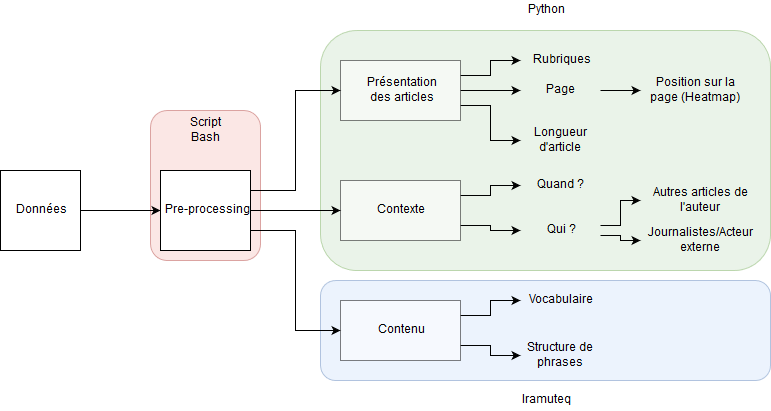
\includegraphics[width=0.7\textwidth]{methodology/methods.png}
\caption{Organisation et outils de l'analyse.}
\label{methods}
\end{figure}

\hypertarget{pre-processing}{%
\subsection{Pre-processing}\label{pre-processing}}

Pour l'explorer de manière plus rapide, nous devons réduire le corpus de
base qui se constitue des articles de la \emph{Gazette de Lausanne}
et du \emph{Journal de Genève} sortis entre 1900 et 1999.

Nous créons trois corpus. Le plus grand est constitué de tous les
articles, décomprimés (du format \texttt{bzip2}) et sans méta-données
concernant la position des mots sur la page. Nous nous servons de ce
corpus-là pour des questions qui regardent l'entièreté des journaux,
comme la longueur en page du journal à une certaine date.

Le deuxième corpus se limite aux articles de caractère financier et est
extrait du premier corpus par la recherche des mots clés suivants:

\begin{itemize}
\item
  secret bancaire
\item
  place financière
\item
  banques suisses
\item
  forfait fiscal
\item
  paradis fiscal
\item
  affaire Chiasso
\item
  argent sale
\item
  blanchiment
\end{itemize}

Nous utilisons ce corpus d'environ 35'000 articles pour nous
comparer avec notre troisième corpus, sélectionné par le seul mot clé
``secret bancaire'', contenant environ 1'700 articles. De cette façon,
nous pouvons déterminer si une certaine tendance de ce corpus est
vraiment signifiante, ou si elle apparaît dans tout le corpus financier.

\hypertarget{statistiques-de-base}{%
\subsection{Statistiques de base}\label{statistiques-de-base}}

Nous commençons en calculant certaines statistiques de base, telles que
le numéro de page, la longueur et la date d'un article. Nous
reproduisons donc le N-Gram dans le temps, pour les articles contenant
``secret bancaire'' par année.

\begin{figure}
\centering
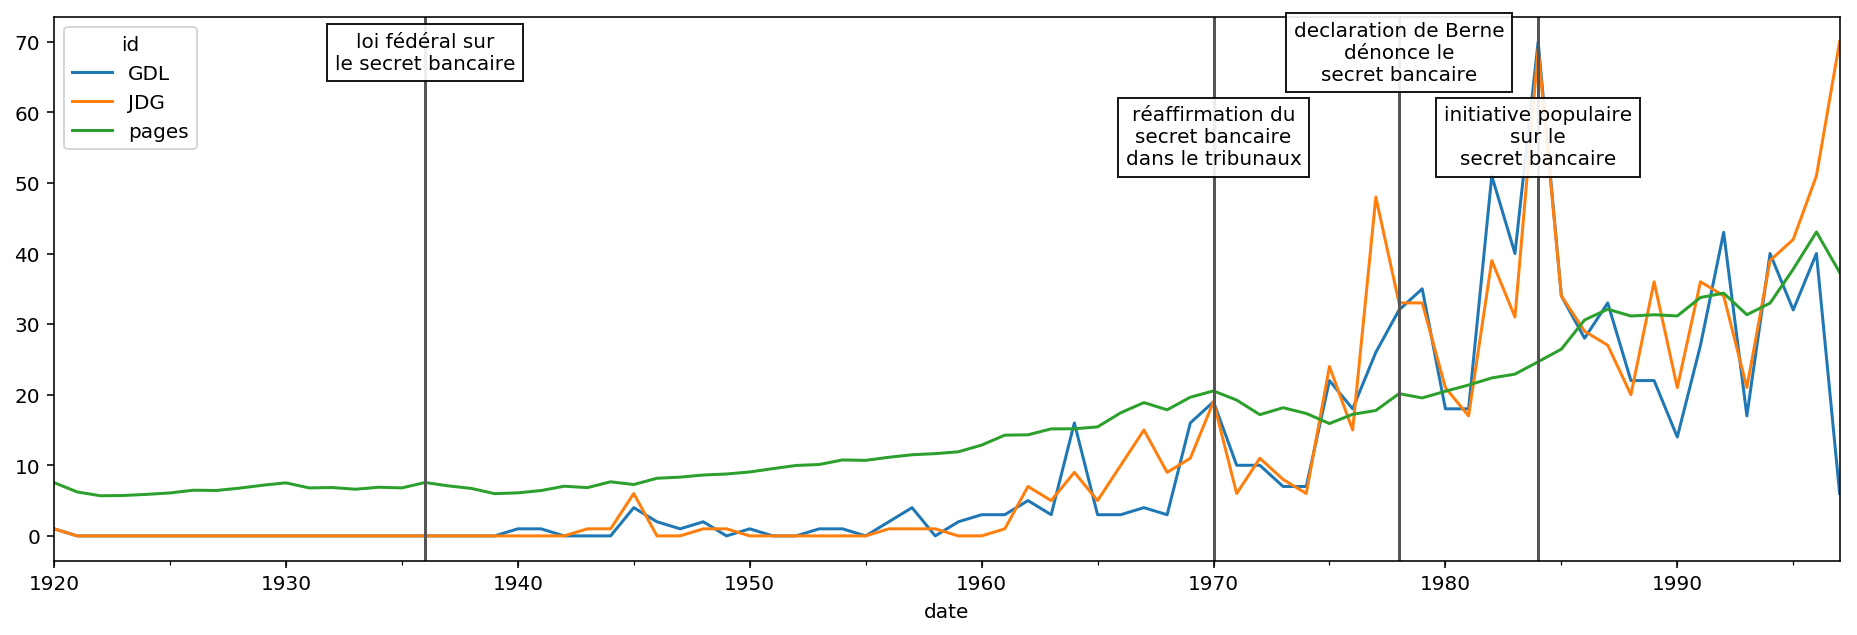
\includegraphics[width=0.7\textwidth]{methodology/ngram_ts.png}
\caption{Apparitions du terme ``secret bancaire'' dans les deux journaux
au cours du temps.}
\end{figure}

Ensuite, nous comparons la longueur d'un article sur le secret bancaire
aux articles génériques du corpus financier. Nous pouvons constater en
regardant l'histogramme suivant que les articles sur le secret bancaire,
dans les deux journaux, sont en général un peu plus longs.

\begin{figure}
\centering
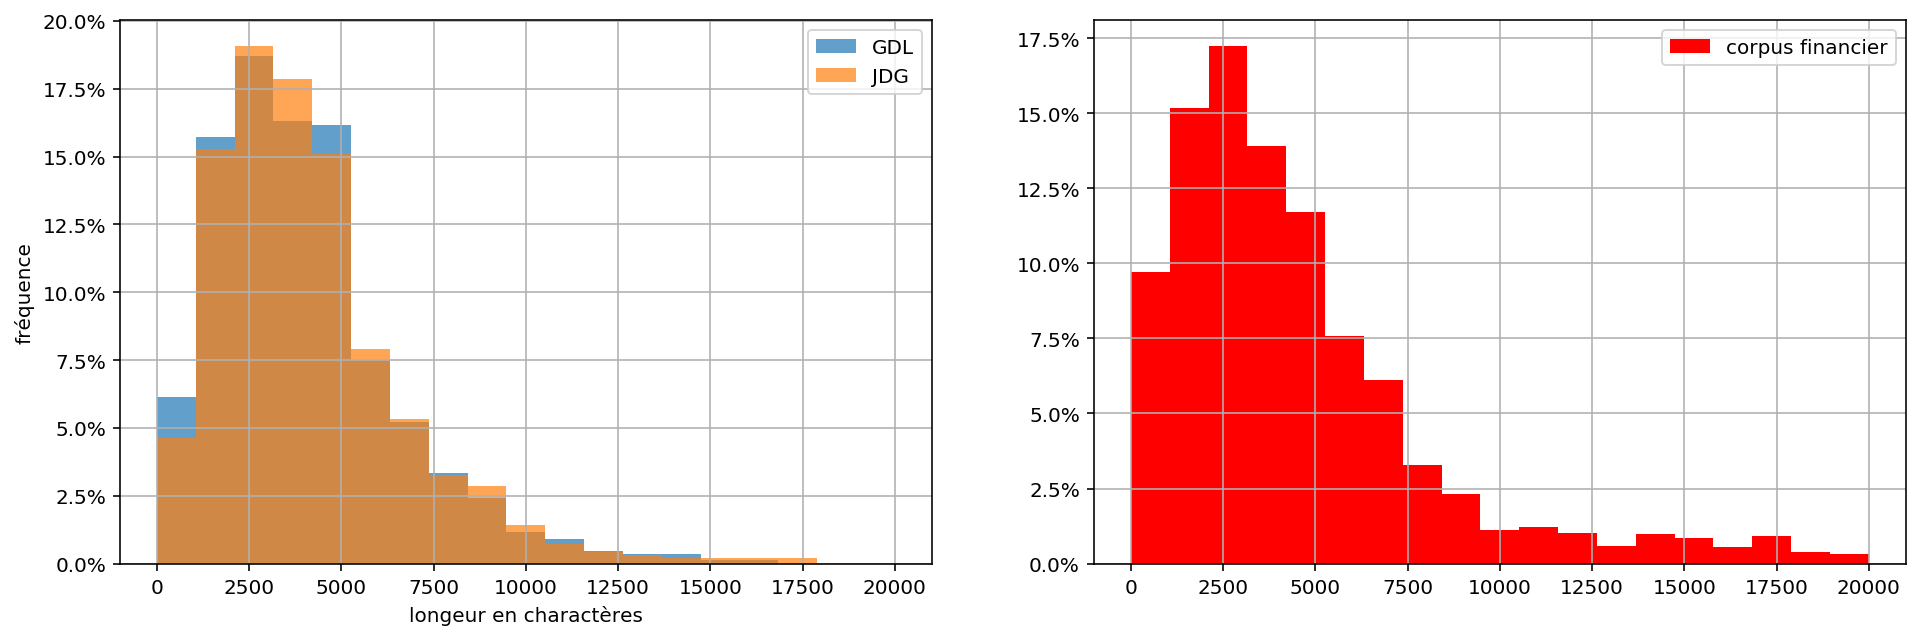
\includegraphics[width=0.6\textwidth ]{methodology/article_lengths.png}
\caption{Distribution de la longueur des articles.}
\end{figure}

Nous examinons aussi, à l'aide d'un histogramme de la page de l'article,
la distribution de la position des articles sur le secret bancaire. Pour
mieux interpréter les résultats de cette analyse, nous trouvons la
longueur du journal pour chaque date et calculons ainsi la position
relative de l'article dans le journal. Nous cherchons enfin à voir si
des rubriques spécialisées traitent le sujet, en examinant des nuages de
points corrélants la date et la page des articles en question. Des ligne
horizontales isolées constituerait un indice d'une rubrique permanente.

\begin{figure}
\centering
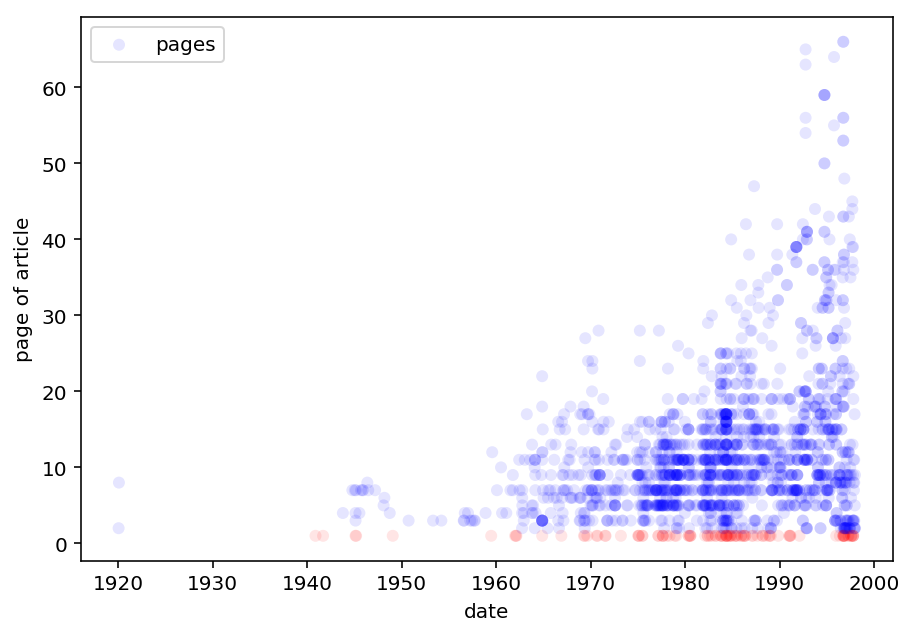
\includegraphics[width=0.5\textwidth ]{methodology/scatter.png}
\caption{Nuage de points de la page des articles dans le temps.}
\end{figure}

En comparant le nombre d'article en première page, nous constatons que
la fréquence d'une première page pour un article sur le secret bancaire
est de 5\% dans la \emph{GDL} et 6\% dans le \emph{JDG}. Alors que la
fréquence d'une première page pour un article générique financier est de
2\% pour la \emph{GDL} et 3\% pour la \emph{JDG}.

\hypertarget{analyse-des-auteurs}{%
\subsection{Analyse des auteurs}\label{analyse-des-auteurs}}

La méta-donnée la plus importante après la date qui est traitée en haut
est l'auteur d'un article. Nous analysons deux catégories d'auteurs.

\hypertarget{agences-de-presse}{%
\paragraph{Agences de presse}\label{agences-de-presse}}

Beaucoup d'articles de journal proviennent d'agences de presse externes
à la rédaction. Nous classifions les articles des agences suivantes:

\begin{itemize}
\item
  ATS: Agence télégraphique suisse
\item
  AFP: Agence France-Presse
\item
  Reuters
\item
  AP: Associated press
\end{itemize}

Ainsi nous trouvons que pour les articles du secret bancaire le taux
d'articles issus d'agences et 10\% plus haut que dans le corpus
financier.

\newpage

\hypertarget{journalistes}{%
\paragraph{Journalistes}\label{journalistes}}

Même si l'auteur n'est pas toujours indiqué -- surtout dans la première
moitié du siècle -- nous arrivons à extraire des données sur les
journalistes. Au moyen d'une liste de noms d'auteurs\footnote{Cette
  liste était obtenue de la page
  \href{https://fr.wikipedia.org/wiki/Journal_de_Gen\%C3\%A8ve}{Wikipédia
  du \emph{Journal de Genève}}.} et des initiales à la fin de l'article,
nous pouvons attribuer des auteurs à plus que 2600 articles.

\begin{figure}
\centering
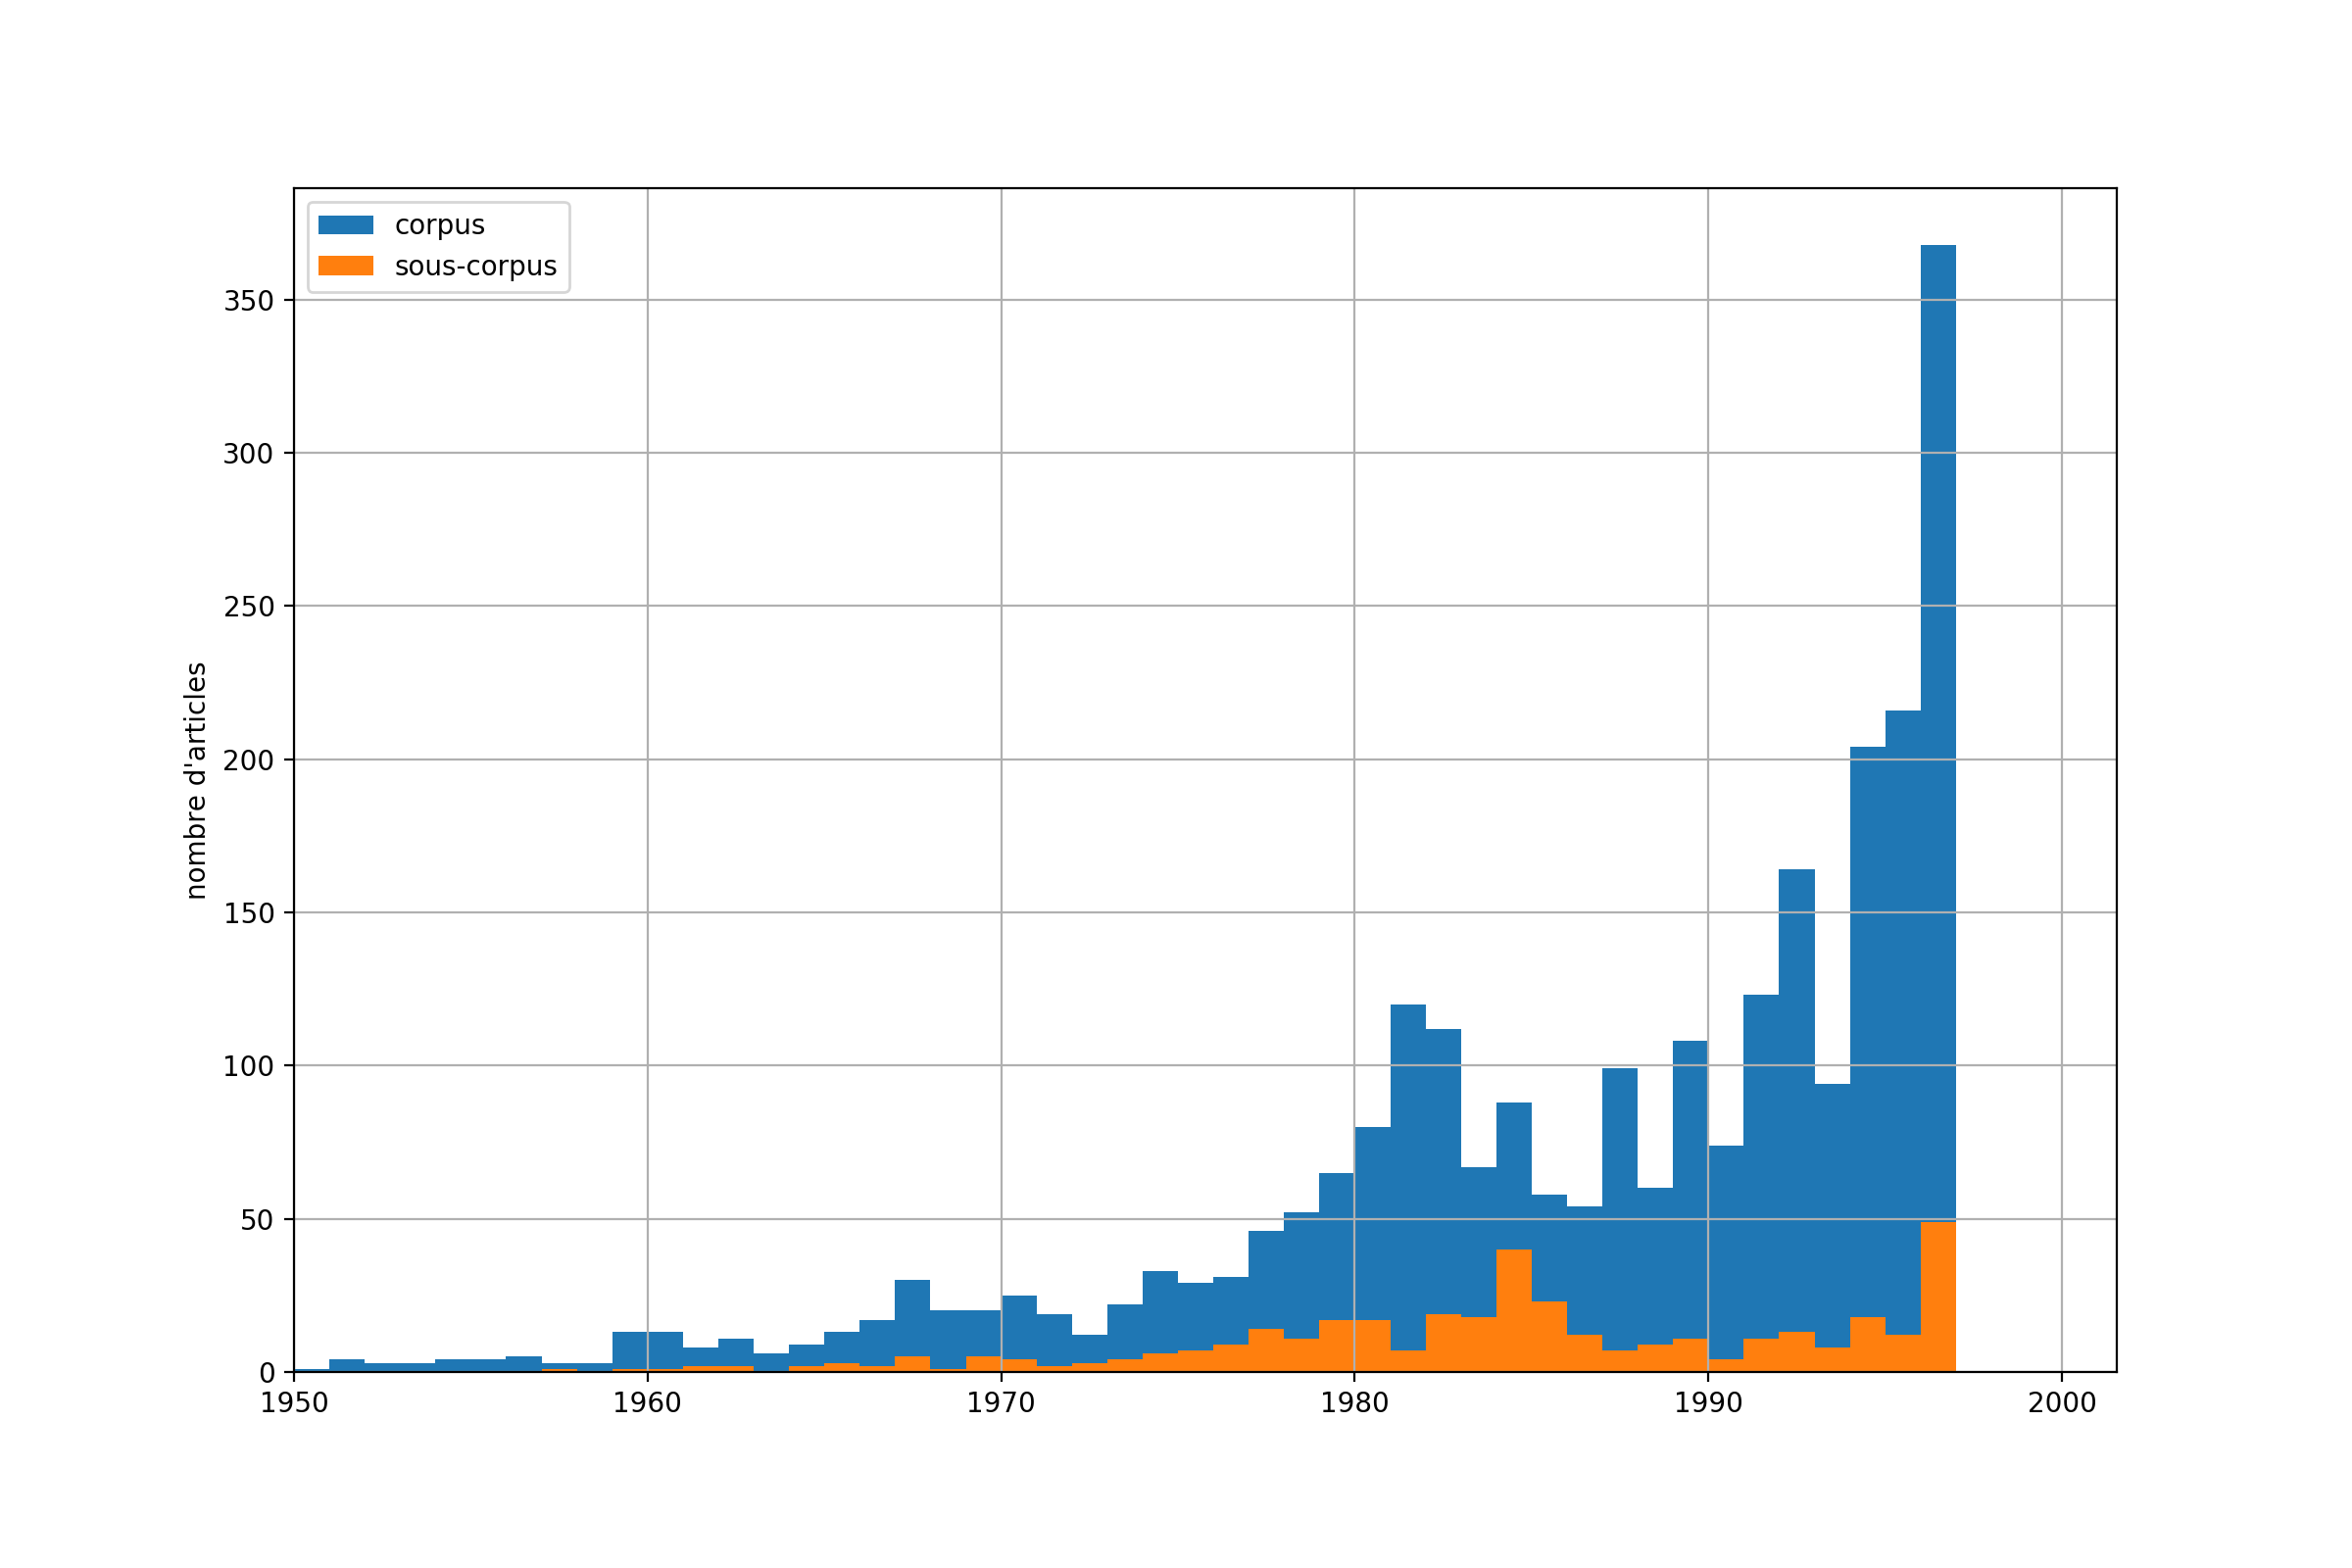
\includegraphics[width=0.6\textwidth]{methodology/author_attributed.png}
\caption{Articles avec auteur attribué.}
\end{figure}

Cette attribution nous permet de poser les questions suivantes: Est-ce
qu'un journaliste est actif dans le deux journaux en même temps? Est-ce
qu'il écrit en moyenne plus souvent sur le secret bancaire que sur
d'autres sujets?

Comme exemple, nous voyons que les deux auteurs du \emph{JDG} qui ont
écrit le plus sur le secret bancaire sont Jean-Luc Lederrey (41
articles) et Jacques-Simon Eggly (29 articles). Les deux sont aussi
actifs dans la \emph{GDL} et cela même avant la fusion des rédactions en
1991. En plus, une recherche LinkedIn ou Wikipédia révèle que les deux
travaillaient aussi dans le monde banquier\footnote{\href{https://ch.linkedin.com/in/lederrey-jean-luc-1456b717}{Jean-Luc
  Lederrey sur LinkedIn}.} ou dans la politique libérale\footnote{\href{https://fr.wikipedia.org/wiki/Jacques-Simon_Eggly}{Jean-Simon
  Eggly sur Wikipédia}.}.

\hypertarget{analyse-du-contenu}{%
\subsection{Analyse du contenu}\label{analyse-du-contenu}}

L'analyse de contenu se limite au corpus ``secret bancaire''. Dans un
premier temps nous produisons des graphiques d'analyses de similitudes
pour les deux journaux.

\begin{figure}
\centering
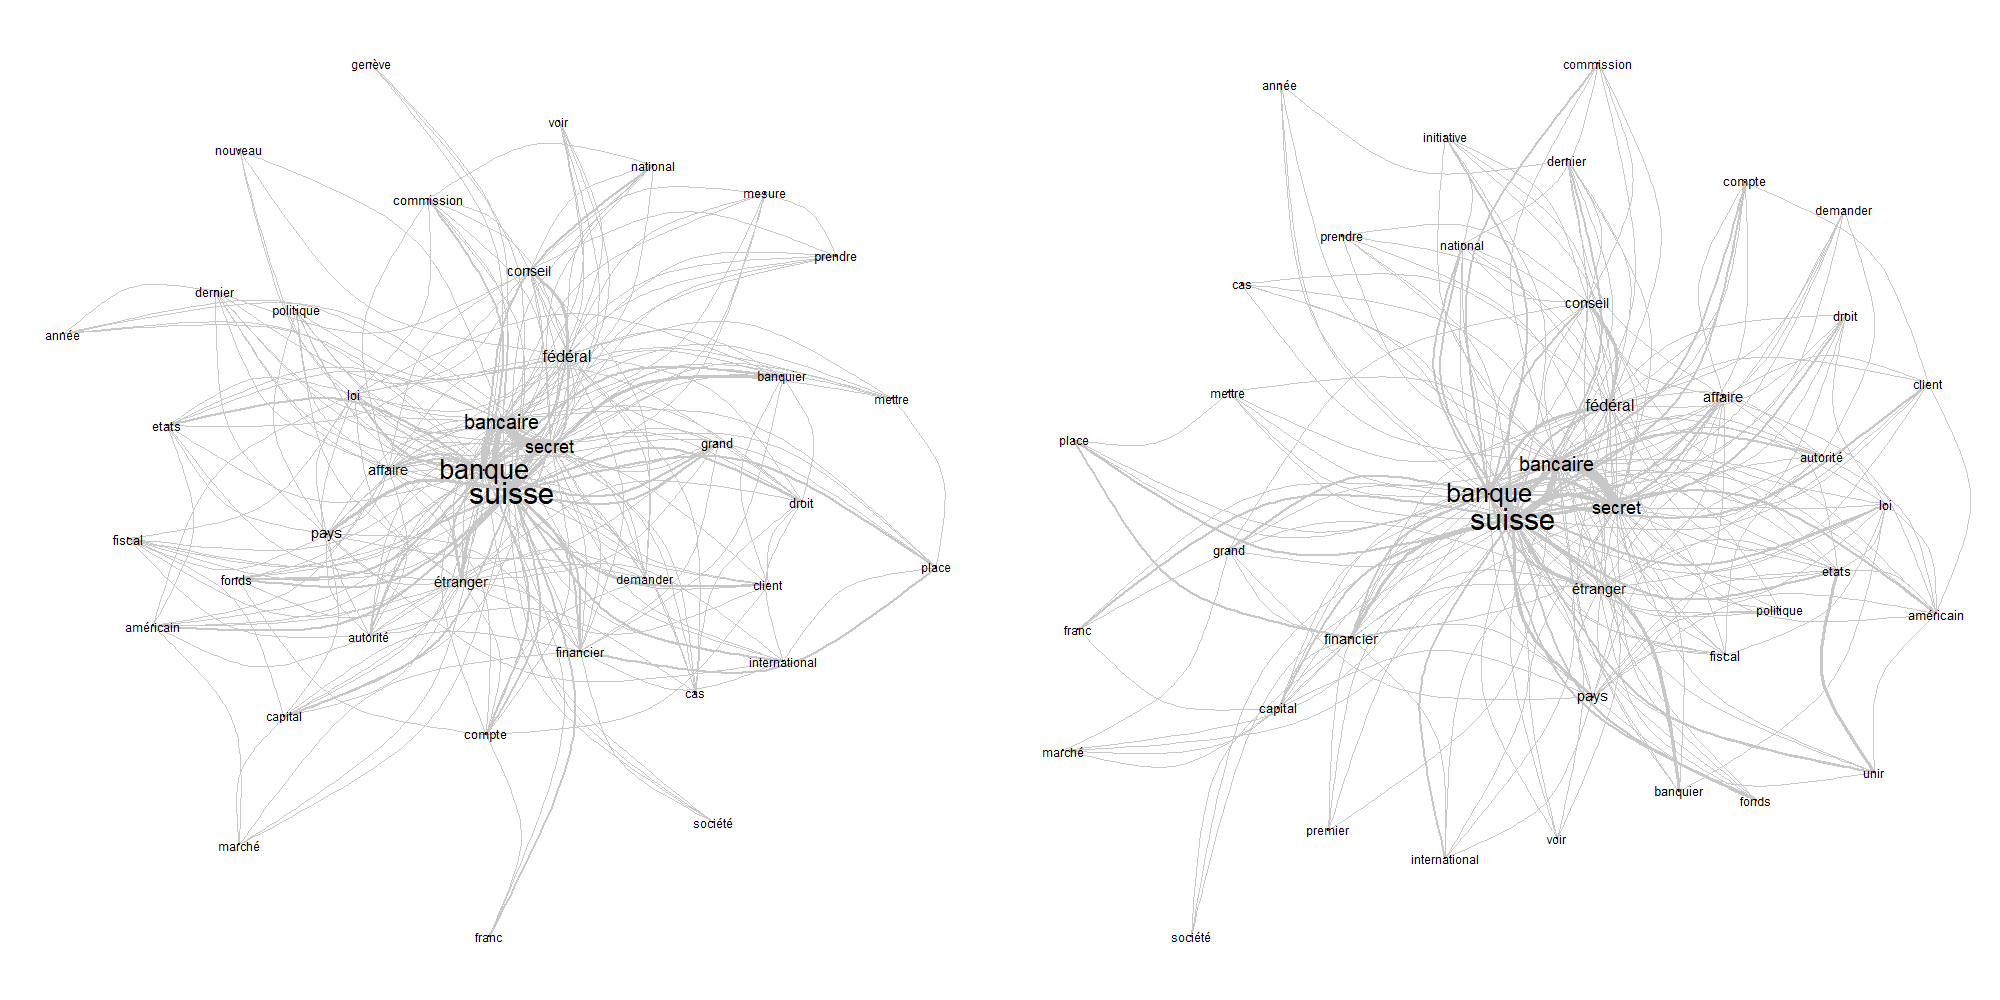
\includegraphics[width=1\textwidth ]{methodology/similitude.png}
\caption{Graphes de similitudes du \emph{JDG} (gauche) et de la
\emph{GDL} (droite).}
\end{figure}

En regardant le résultat on voit que les mots qui apparaissent souvent
avec ``secret bancaire'' dans les textes de la \emph{GDL} et du
\emph{JDG} sont différents. Pour la \emph{GDL} on voit des mots tel que
``affaire'' qui apparaissent et qu'on ne voit pas dans le résultat avec
le \emph{JDG}.

Afin de rendre les visuels utilisables, nous affichons ici seulement 40
mots (autres que préposition et déterminants). Afin de ne pas surcharger
l'image, seuls les termes qui apparaissent plus de 50 fois ensemble sont
montrés reliés dans le graphe.

En suite, toujours dans un esprit de comparaison des journaux, nous
produisons deux dendrogrammes sur les journaux.

\begin{figure}
\centering
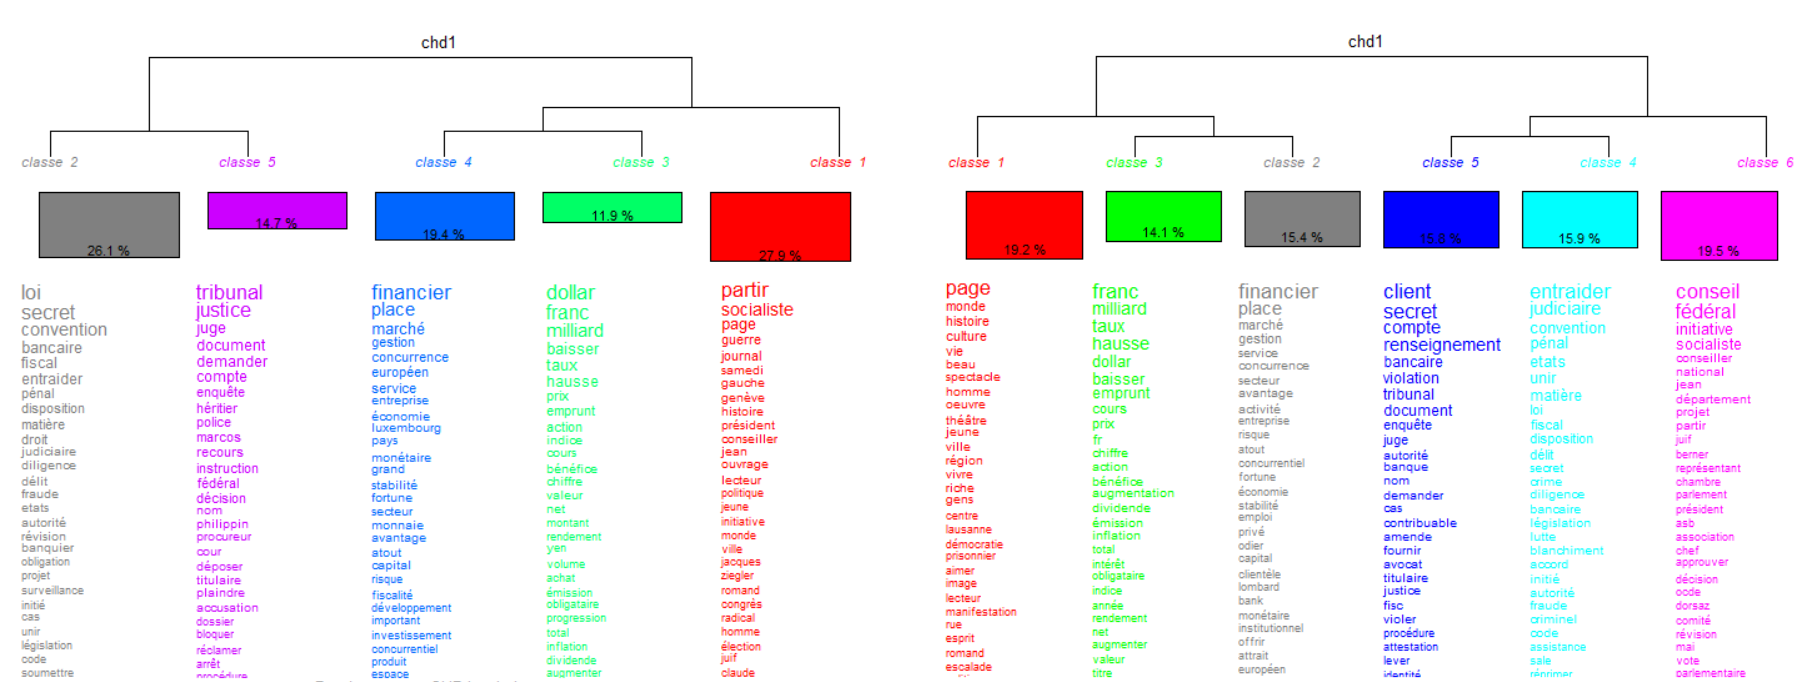
\includegraphics[width=1\textwidth ]{methodology/dendrogram.png}
\caption{Dendrogrammes du \emph{JDG} (gauche) et de la \emph{GDL}
(droite).}
\end{figure}

Cela nous permet de comparer le langage utilisé dans les deux journaux,
nous voyons qu'un journal a été organisé en cinq clusters et l'autre en
six, montrant une divergence dans la façon d'aborder le sujet. Les
champs lexicaux sont proches mais cela nous n'apporte encore rien sur le
contexte d'utilisation des mots.

Avec ces informations, nous pouvons déjà observer que le style
d'écriture des articles est différent. Nous observons par exemple que la
\emph{GDL} semble mettre ensemble des articles qui parlent de secret
bancaire avec des articles qui parlent d'affaires judiciaires (avec les
mots ``secret'', ``bancaire'' proche du mot ``judiciaire'').

\hypertarget{critique-et-difficultuxe9es}{%
\subsection{Critique et
difficultées}\label{critique-et-difficultuxe9es}}

Notre analyse est particulièrement perturbée par les problèmes de l'OCR
de basse qualité. Car, les termes que nous tentons d'isoler sont plutôt
long et une erreur de reconnaissance est bien plus probable.

Un autre problème est que le format de reconnaissance des articles est
assez limité. Il a fallu que nous allions chercher le nom des auteurs
manuellement, cependant nous avons observé que mettre le nom de l'auteur
sur un article de journal ne devient courant qu'à partir des années 60,
limitant nos capacité d'analyse avant cette période.

Nous avons réussi à contourner ce problème en utilisant une liste de
noms de journalistes ayant travaillé pour le \emph{JDG}. Cependant nous
n'avons pas trouvé une telle liste pour la \emph{GDL}.


\hypertarget{analyse}{%
\section{Analyse}\label{analyse}}

\hypertarget{intuxe9ruxeat-des-journaux-au-sujet-du-secret-bancaire}{%
\subsection{\texorpdfstring{Intérêt des journaux au sujet du
\emph{secret
bancaire}}{Intérêt des journaux au sujet du secret bancaire}}\label{intuxe9ruxeat-des-journaux-au-sujet-du-secret-bancaire}}

Le sujet du secret bancaire a suscité une centaine de premières pages au
sein des deux journaux de 1940 jusqu'à la fin des années 90. Ce chiffre
relativement petit nous permet de lire quelques premières pages pour
mieux mettre en contexte nos autres analyses.

De manière générale et excluant l'année 1984 de l'initiative populaire
au même sujet, le secret bancaire n'est pas un sujet très important dans
le corpus financier. Le sous-corpus ``secret bancaire'' ne constitue que
5\% des articles du corpus financier, qui lui-même ne contient qu'une
petite partie de tous les articles. Il est remarquable que dans le
sous-corpus la proportion d'articles qui proviennent d'agences de presse
est de dix pour-cent plus élevée que dans le corpus financier (29\% pour
le ``secret bancaire'', 18\% pour le financier). Cela pourrait être
justifié par l'hypothèse que le sujet a peu d'importance pour les
rédactions, qui n'utilisent souvent que des dépêches pour en parler.
Comme le montre le collage \ref{depeches}, les dépêches parlent surtout
de cas judiciaires et de petits scandales.

\begin{figure}
\centering
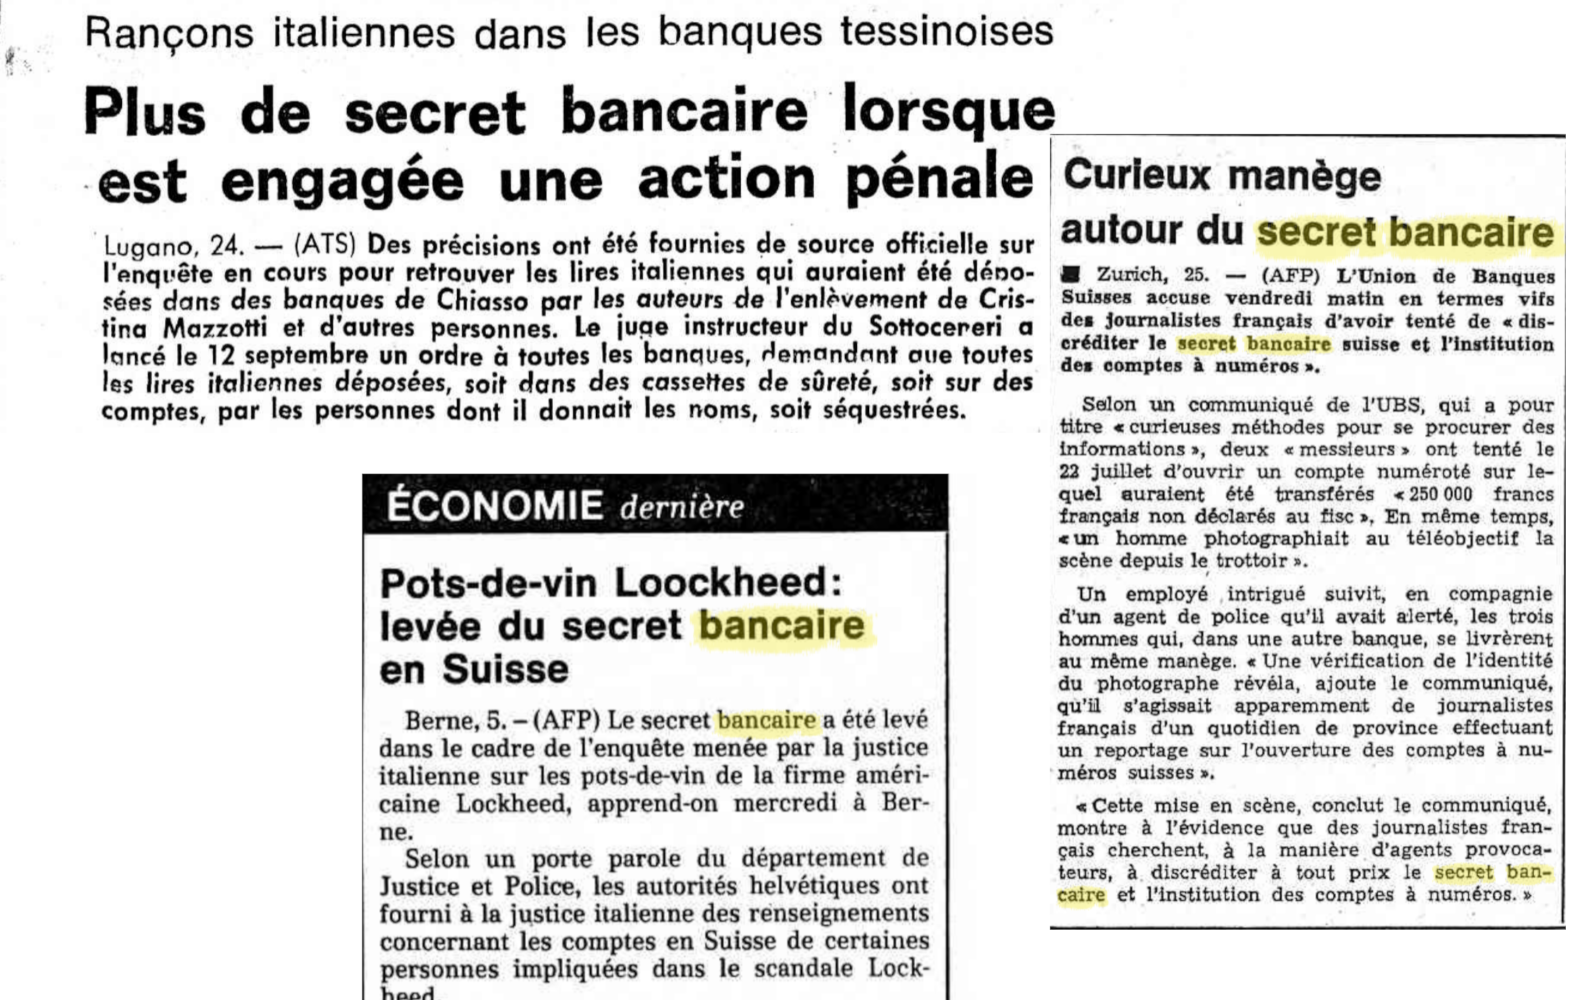
\includegraphics[width=0.8\textwidth ]{analysis/agencies_collage.png}
\caption{\label{depeches} Exemple de dépêches, suisses et étrangères.}
\end{figure}

Pour cerner l'origine de cet intérêt, nous comparons la fraction de
dépêches venant de l'étranger à celles de l'Agence télégraphique suisse
(ATS). La figure \ref{percentage1} montre comment cette fraction évolue
dans le sous-corpus au cours du temps. Nous trouvons deux périodes où
les dépêches étrangères ont une certaine présence: 1972 -- 1977 et 1986
-- 1992. Ce sont des périodes relativement calmes, où à l'intérieur de
la Suisse le sujet n'est pas d'actualité. Les dépêches dans le collage
\ref{depeches} représentent bien le type d'article sur des faits mineurs
apparaissant dans cette période calme.

\begin{figure}
\centering
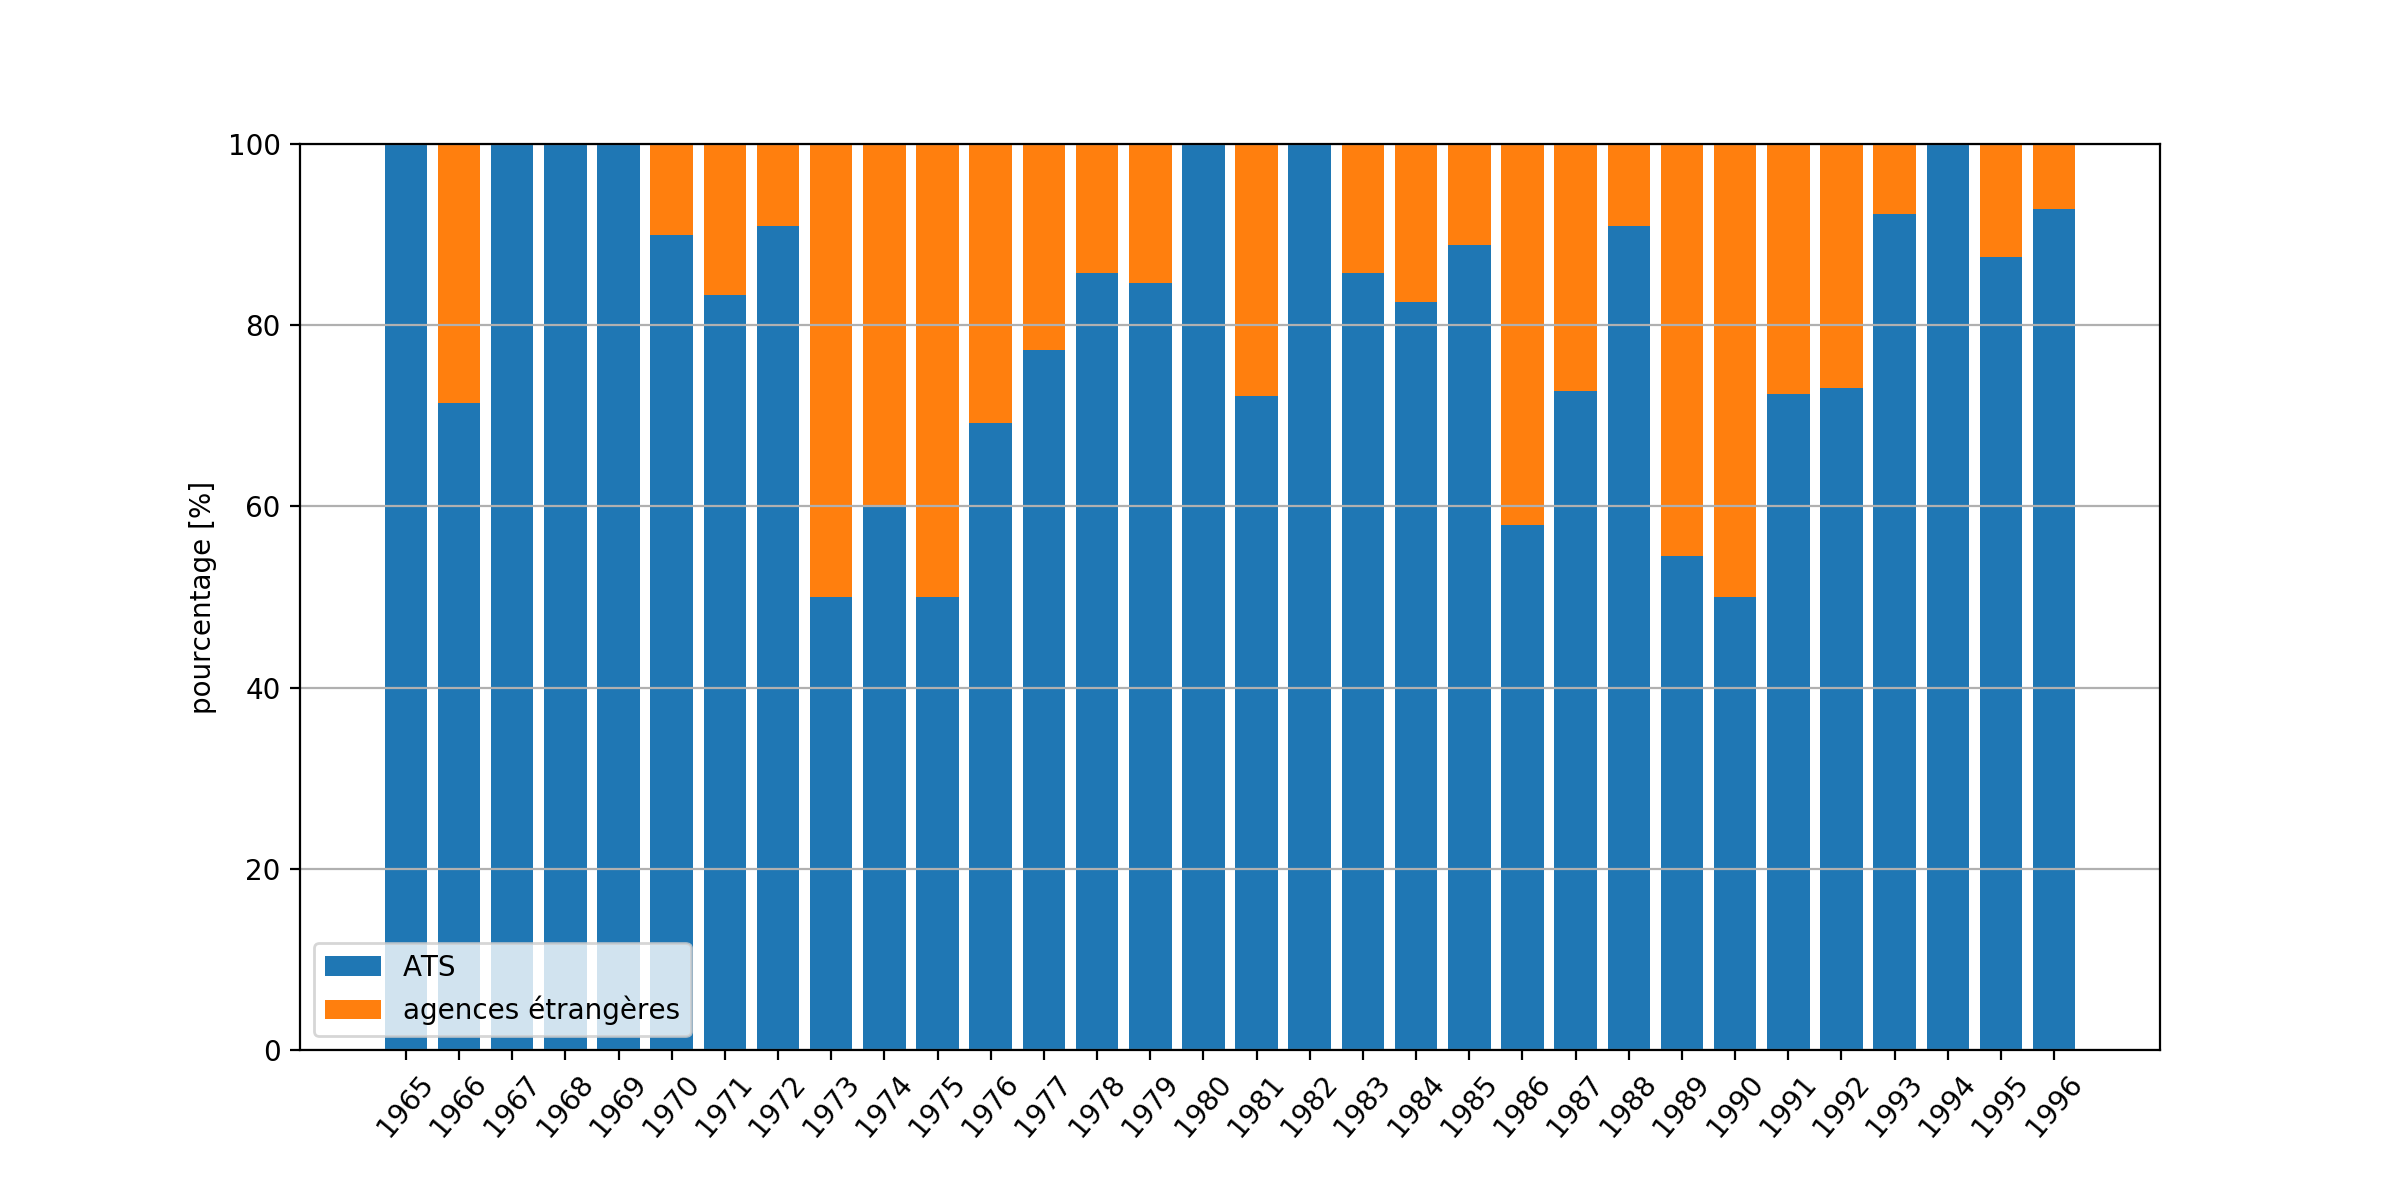
\includegraphics[width=0.7\textwidth ]{analysis/agency_percentage.png}
\caption{\label{percentage1} Distribution relative des articles
d'agences de presse étrangères pour le ``secret bancaire''.}
\end{figure}

La série temporelle du nombre d'articles par catégorie d'auteur (fig.
\ref{categorie}) met en évidence une nette chute de l'utilisation de
dépêches étrangères qui parlent du secret bancaire pendant exactement la
période avant la votation de 1984. Vue la forte orientation politique
des deux rédactions contre l'initiative, on peut supposer que les
articles d'agences étrangères qui ne concernent pas l'initiative sont
minimisés, pour ne pas détourner l'attention des lecteurs.

\begin{figure}
\centering
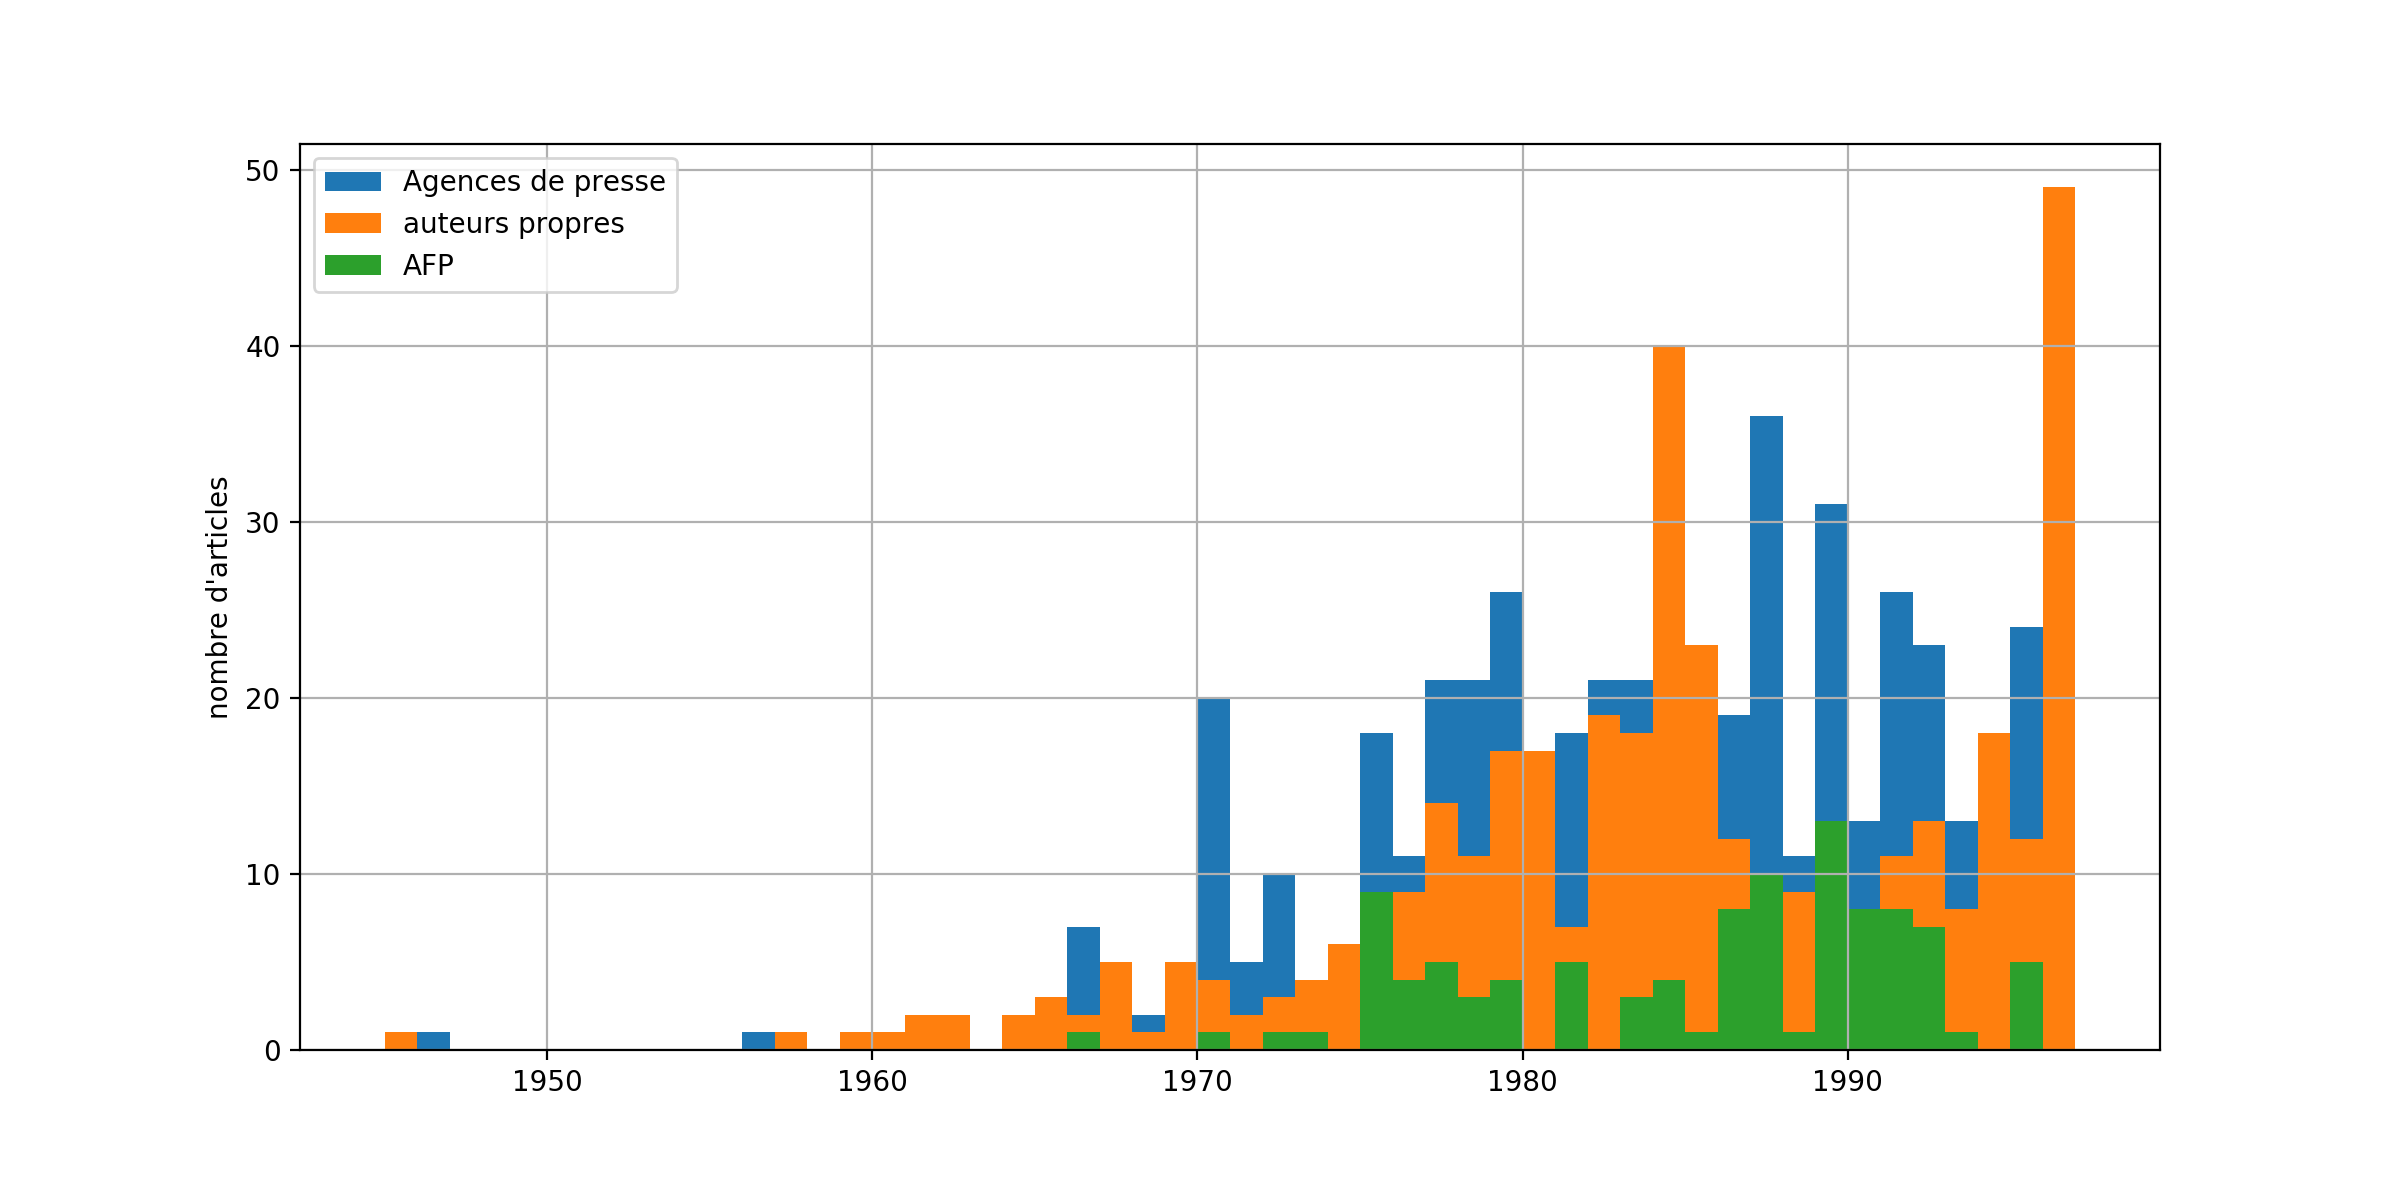
\includegraphics[width=1\textwidth ]{analysis/authors_agency_count.png}
\caption{\label{categorie} Nombre d'articles par catégorie d'auteur au
cour du temps.}
\end{figure}

Par la lecture des premières pages, nous trouvons le ensemble suivant de
périodes principales dans l'histoire du secret bancaire:

\begin{itemize}
\item
  1940--45: Le secret bancaire est menacé de l'intérieur par le
  gouvernement, à cause de l'économie de guerre, et de l'extérieur par
  les futures nations unies, qui désirent l'entraide judiciaire et
  fiscale.
\item
  1946--65: Période de calme où aucune attaque importante n'est montée
  contre le secret bancaire. Quelques frictions avec la France se
  résolvent en une impasse.
\item
  1966--70: Tensions et efforts diplomatiques avec les États-Unis, qui
  critiquent durement le secret bancaire qui leur empêche d'enquêter
  efficacement la criminalité organisée. Cela se résout avec des accords
  bilatéraux qui concèdent très peu à la justice américaine.
\item
  1975--84: Tumultes intérieurs vis au secret bancaire. L'économie en
  récession et la force du Franc Suisse dans les marchés de devises
  portent les milieux politiques socialistes à attaquer le secret
  bancaire comme responsable. Le débat intérieur continue jusqu'en 1984,
  quand l'initiative socialiste contre le secret bancaire est repoussée.
\item
  1987--89: Pressions américaines poussent la Suisse à approuver la
  levée du secret bancaire dans le cas de manipulation des marchés
  (\emph{insider trading}), un délit qui n'était pas persécuté en Suisse
  jusqu'alors.
\item
  1996--suite: Affaire des fonds juifs en déshérence. Le conseil
  national vote à l'unanimité pour la levée du secret bancaire pour la
  commission Bergier.
\end{itemize}

La tonalité du discours dans les deux journaux au cours de ces périodes
est surtout intéressante. Dans la première période, le ton est positif
et tranquille. En 1975, le ton change rapidement: des articles écrits
par Marian Stepcinsky, Jean-Luc Lederrey, et par le futur politicien
libéral Jacques-Simon Eggly gagnent souvent la première page. Ces
articles sont des pièces d'opinion, souvent virulentes, où les avantages
du secret bancaire sont rappelés. Contrairement aux périodes
précédentes, où ces avantages ont été considérés trop évidents pour les
souligner. Ces articles d'opinion forment une véritable propagande en
faveur du secret bancaire et contre les socialistes, et donnent de
précises indications de vote dans le mois avant l'initiative.

\begin{figure}
\centering
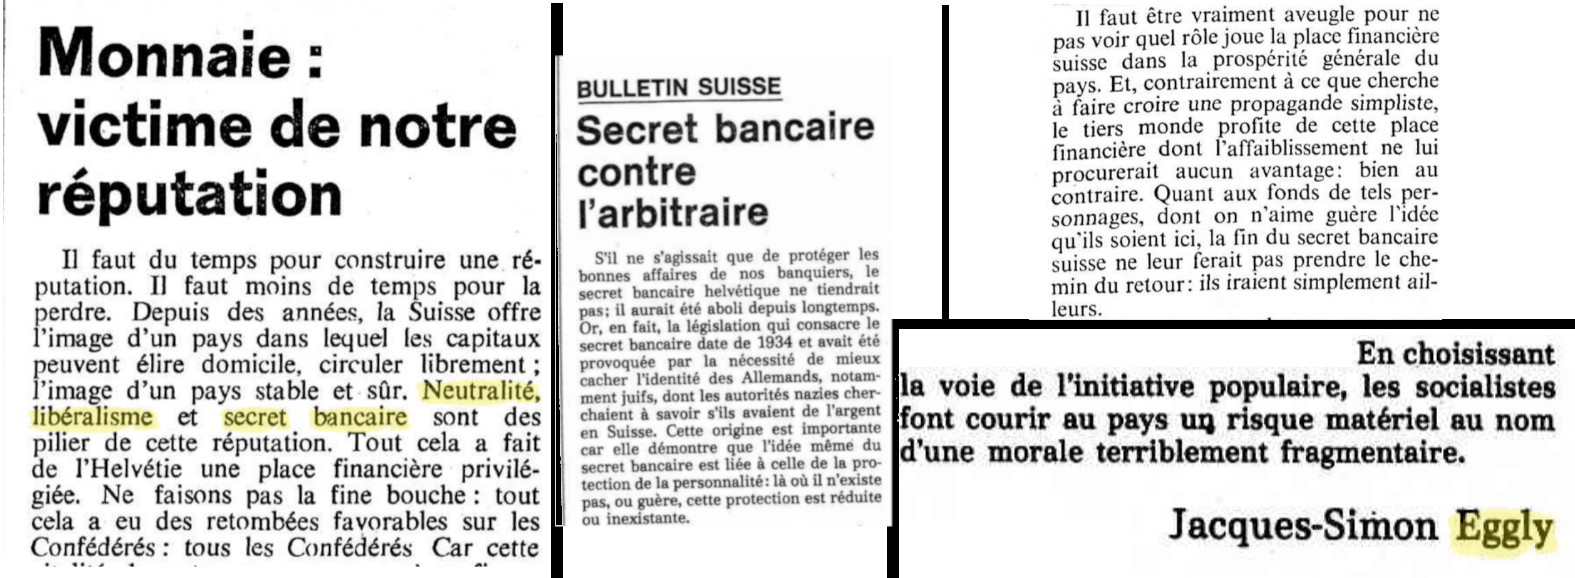
\includegraphics[width=0.9\textwidth ]{analysis/propaganda_collage.png}
\caption{\label{propagande} Exemple d'articles partisans apparus dans la
période de l'initiative.}
\end{figure}

La tonalité des articles redevient enfin plus descriptive et
s'assouplie, après que l'initiative soit rejetée. Les lois sur la
manipulation des marchés et la commission Bergier ne sont pas perçues
comme menace essentielles à la stabilité de la place financière.

\hypertarget{comparaison-des-deux-journaux}{%
\subsection{Comparaison des deux
journaux}\label{comparaison-des-deux-journaux}}

En isolant les articles contenant ``secret bancaire'', nous avons
auparavant isolé les articles en différents groupes avec la méthode de
Reinert. La première chose que nous remarquons est qu'entre les deux
journaux nous obtenons des groupes différents. Afin de mieux comprendre
comment les articles sont classés, nous avons aussi effectué des
Chi²-tests sur des mots-clés. Par exemple dans le \emph{Journal de
Genève}, nous pouvons voir que le terme ``UBS'' va éloigner l'article du
groupe contenant les termes plus proches du sujet, comme ``secret'',
``convention'', ``droit'' ou ``judiciaire'' que l'on voit dans la
première classe du dendrogramme (voir partie méthodologie). Cela pousse
l'article fortement vers le groupe trois qui contient des termes assez
descriptifs (sur les intérêts et les devises).

\begin{figure}
\centering
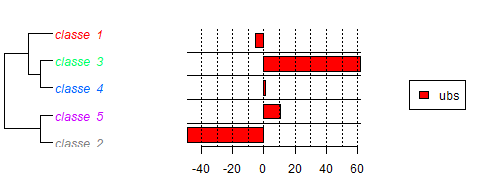
\includegraphics[width=0.9\textwidth ]{analysis/chiubs.png}
\caption{Chi²-Test du terme ``UBS'' dans le \emph{JDG}.}
\end{figure}

D'autres tests similaires pointent vers d'autres divisions, ou les
articles utilisants des termes juridiques et/ou techniques précis (comme
``bancaire'', ``fraude'', ``autorité'') vont concentrer les articles
dans une même classe. Mais nous voyons aussi que les termes qui ramènent
au nom des banques sont dissociés des groupes parlant de l'actualité du
secret bancaire.

Du côté de la \emph{GDL}, nous trouvons six groupes. Là ou le \emph{JDG}
semble avoir des classes qui sont basées sur des sujets différents
(économie, affaires judiciaires, légal), dans la \emph{GDL} il semble
que les événements marquants de la période génèrent plus d'attention.
Car, on retrouve une classe avec des mots rappelant des affaires
judiciaires. Dans cette classe on retrouve des termes tels que
``renseignement'', ``tribunal'', ``violer''\ldots{} Cela semble indiquer
que les différents scandales entourant le secret bancaire sont perçus
comme plus importants dans la \emph{GDL} que le \emph{JDG}. Cependant,
ici comme dans le \emph{JDG} le nom des banques suisses apparaît plutôt
dans le groupe d'articles référençant des termes financiers plus
généraux: la classe 3, qui est très similaire à la classe 3 dans
l'analyse du \emph{JDG} (avec les noms de devises et des quantités).

\begin{figure}
\centering
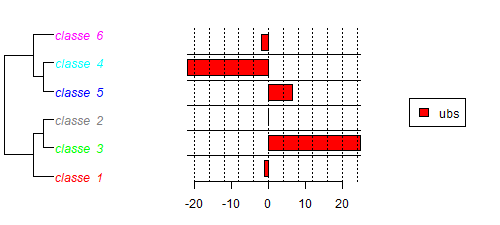
\includegraphics[width=0.9\textwidth ]{analysis/ubs_chisquare_gdl.png}
\caption{Chi²-Test du terme ``UBS'' dans la \emph{GDL}.}
\end{figure}

Tout ceci semble indiquer que, même si l'emphase apportée aux différents
événements entourant le secret bancaire est différente entre les deux
journaux, les deux semblent aussi dissocier les banques du sujet même du
secret bancaire.

\hypertarget{conclusions}{%
\subsection{Conclusions}\label{conclusions}}

Cette analyse du sujet évidence clairement l'adhésion des deux
rédactions à la politique libérale. L'absence de dépêches étrangères,
surtout centrées sur les scandales, pendant la période de l'initiative
peut être considérée comme une forte indication du rôle politique des
deux journaux.

L'analyse linguistique nous montre que la \emph{GDL} donne plus
d'importance aux affaires concrètes et le \emph{JDG} plus au coté
abstrait législatif, bien que aucun des deux journaux ne pointe jamais
du doigt. Dans les deux journaux, le secret bancaire est abordé dans un
contexte politique plutôt que financier, en défendant ces principes à la
base plutôt qu'en montrant les inconvénients qu'il cause aux fiscs et
aux investigateurs internationaux.



\newpage

\bibliographystyle{chicago}
\bibliography{1_semester/bib/bibliography}

\end{document}
